\documentclass[../TDO3.tex]{subfiles}%

\begin{document}
\section[s]"1"{Constructions optiques de miroirs}

\QR{%
	Dans chacune des situations suivantes, déterminer la nature des faisceaux,
	nommer les intersections dessinées, compléter la marche des rayons lumineux et
	commenter la nature de l'objet et de l'image.
	\begin{center}
		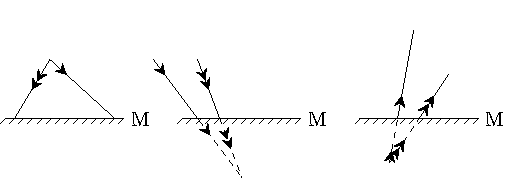
\includegraphics[height=4cm]{miroir_plan}
	\end{center}
}{%
	~
	\smallbreak
	\vspace{-15pt}
	\begin{tcn}[tabularx={Y|Y|Y}](data){Schéma}
		&&\\
		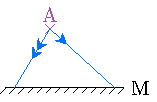
\includegraphics{td3-2-1a} &
		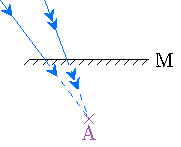
\includegraphics{td3-2-2a} &
		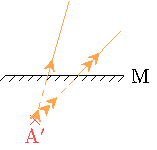
\includegraphics{td3-2-3a}\\
		Les rayons, incidents, se coupent avant le miroir. &
		Les rayons, incidents, se coupent après le miroir. &
		Les rayons, émergents, se coupent après le miroir.\\
	\end{tcn}
	\begin{tcbraster}[raster columns=2, raster equal height=rows]
		\begin{tcn}[](ques){Résultat attendu}
			Construire les objets et images avec les règles du miroir plan.
		\end{tcn}
		\begin{tcn}[](tool)'r'{Outils}
			Image par miroir plan = symétrique. Objet à intersection des indicents,
			image intersection émergents.
		\end{tcn}
	\end{tcbraster}
	\begin{tcn}[tabularx={Y|Y|Y}](appl){Application}
		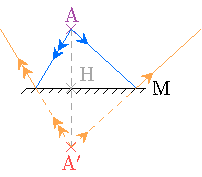
\includegraphics{td3-2-1b} &
		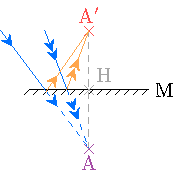
\includegraphics{td3-2-2b} &
		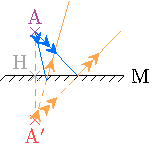
\includegraphics{td3-2-3b}\\
		Le symétrique de A donne A' où les rayons émergents se croisent. &
		Le symétrique de A donne A' où les rayons émergents se croisent. &
		Le symétrique de A' donne A où les rayons incidents se croisent.\\
		A est réel, A' virtuel. &
		A est virtuel, A' réel. &
		A est réel, A' virtuel.\\
	\end{tcn}
}
\end{document}
